\documentclass[twocolumn,10pt]{article}
\usepackage{amssymb}
\usepackage{amsmath}
\usepackage{amsfonts}
\usepackage{array,url,kantlipsum}
\usepackage{lineno,hyperref}
\usepackage{graphicx}
\usepackage{float}
\graphicspath{{./Figures/}}
\usepackage[margin=0.75in,tmargin=1in,bmargin=1in]{geometry}
\usepackage{array,multirow}
\usepackage{multirow}
\usepackage{tabu}
\usepackage[table]{xcolor}

\begin{document}
\twocolumn[{%
 \centering
 \LARGE Smart Recipe Measurements with Learned Volume Prediction \\[0.5em]
 \large By Samantha Maticka and Kurt Nelson \\[1em]
 \normalsize
}]

\begin{abstract}
In this work we present the implementation of computer vision and machine learning to teach phones how to measure the volume of a poured liquid from video recordings. The ultimate goal is to develop a mobile application that removes the need for measuring cups in the kitchen by autonomously 1) storing ingredient measurements while food preparation is underway, or 2) instructing users on when to stop adding a particular ingredient. Experiments for data collection and feature extraction are outlined. We then present a model development and selection process that is applied to numerous regression and classification models for both volume prediction as a continuous random variable, and as a classification problem with labels increment in 1/4 cups. Of the regression models tested, locally weighted least squares regression performed best, with a test-data root mean squared error of 0.13 cup. For the classification models, Softmax regression performed best with a missclassification error of 25\%. Both models reduced prediction errors by a factor of 3 relative to approximate physics estimates.        
\end{abstract}

\section{Introduction}
Would you rather chew off your pinky finger or measure ingredients for the rest of your life? The response is unanimous; pinky's are overrated anyhow. No one likes measuring ingredients, but the Italian Grandma Method (IGM), adding a splash of this and a dab of that, produces gastronomical disasters for all but the most experienced chefs (e.g. IG’s). Many of us casual cooks are unable to reproduce winning recipes when applying the IGM, and instead are left with a one-hit-wonder followed by an onslaught of failed recreation attempts that litter our refrigerators with dreadful leftovers.

Can machine learning help solve this dystopia? Predictive algorithms are already heavily embedded in the restaurant industry through mobile application like Yelp or Uber Eats, where user can easily access predicted restaurant suggestions, seating times, and even food delivery times. Machine learning is also finding its way into the common kitchen. An extensive body of literature is dedicated to statistical inference of recipe recommendation \cite{freyne2010,forbes2011,ueda2011,kamieth2011}. Discriminative classifiers are even being used to rank computer generated, "computational creative" recipes \cite{cromwell2015}. Machine learning may even one day replace human chefs with a robotic alternative \cite{Moley2014}. Although many exciting machine learning cooking- and food preparation-based applications are available, to the best of our knowledge machine learning has not been directly applied to guide humans through ingredient measuring.   

Fear not, the world of cooking will soon be a better place. By applying machine learning, we aim to solve this dystopia by creating a mobile application that uses live video recordings to autonomously 1) measure and record ingredients during meal preparation, or 2) guide causal cooks through recipes by instructing when to stop adding a particular ingredient. The ultimate goal is to remove measuring cups form the kitchen. As an initial development step, this paper outlines the application of machine learning and computer vision to teach phones how to  autonomously measure poured liquids. The problem is approached from both a regression and classification standpoint. Predicting poured volumes as a continuous random variable is necessary to instruct users on when to stop poring, while recipe recording requires pour classification. In the remainder of this paper we outline a data collection and feature extraction technique relevant to volume prediction (Section~\ref{Data collection}), then present a model development and selection process (Section~\ref{mdoel selection}) which is applied to both the regression (Section~\ref{regression}) and classification problem (Section~\ref{classifcation}).  

\section{Physics-based prediction}
Although machine learning has not been applied to measurement predictions in the kitchen, the volume of a poured liquid $V$ can be exactly computed from basic fluid dynamics if the velocity $v(x,y,t)$, cross-sectional area $A(x,y,t)$, and pour duration are known, viz. 
\begin{equation} \label{eq:1}
V = \iiint v(x,y,t) A(x,y,t) dx dz dt \\.
\end{equation}
Here, both $v(x,y,t)$ and $A(x,y,t)$ are spatially and temporally dependent and must be evaluated a fixed height $z$. The challenge in making physical volume predictions is exactly measuring $v(x,y,t)$ and $A(x,y,t)$. However the calculation can be simplified if a representative time- and spatially-averaged area $A$ and velocity $v$ can be approximated over the pour duration $T$, giving $V = AvT$ (note: time- and spatially-averaged variables are indicated by the absence of $(x,y,t)$). Although these variables can be approximated from video footage using simple computer vision techniques, the approximations are often crude. However, the physical volume prediction can be improved by introducing a fitting coefficient $\alpha$, 
\begin{equation} \label{eq:2}
V = \alpha AvT \\.
\end{equation}
Physically $\alpha$ represents a correction factor that partially accounts for approximation errors for $v$, $A$, and $T$, and encompasses the required constant for an area prediction (i.e. includes a factor of $\pi/4$ if the cross-sectional area of the stream is truly a circle). We take the volume prediction given by Equation~(\ref{eq:2}) as a baseline estimate for which we compare our machine learning algorithms against. For the classification problem, the volume prediction is rounded to the nearest quarter cup. Additional details on how $\alpha$ is computed are given in Section~\ref{regression}.  

\section{Data collection and feature extraction}
\label{Data collection}
Data was collected by filming over 250 videos of pre-measured water (about 20 video samples per volume, with volumes ranging from 1/4 cups (c) to 2 1/4 c, in 1/4 c increments). The experiments were kept highly controlled to minimize error resulting from experimental setup. Lighting was positioned to reduce glares and shadowing, and a ruler was included in all videos to calibrate pixel length. The water was also dyed blue to enhance color contrast. 

The videos were then processed to extract the 3 fundamental features ($A$, $v$, and $T$). Each film was broken into a series of still frames. To estimate $T$, the time difference between frames containing the stream start and stop was calculated. These frames were found by first computing the Frobenius matrix norm of the pixel intensity difference between consecutive images, then defining the frames by the first time the norm exceeded (start) and then dropped below (stop) a set threshold (red dots in Figure~\ref{fig:ImageIntensity}).

\begin{figure}
\centering
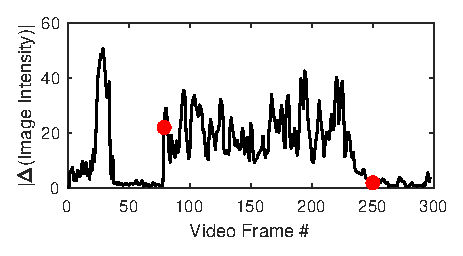
\includegraphics[width=80mm]{ImageIntensity}
\caption{Frobenius matrix norm of the pixel intensity difference used as an indicator of the stream start and stop times (red dots).}
\label{fig:ImageIntensity}
\end{figure}

\begin{figure}
\centering
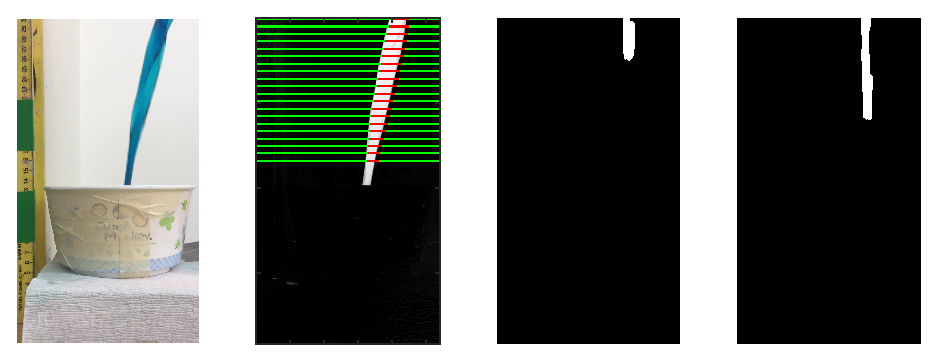
\includegraphics[width=80mm]{LengthScaleExtraction}
\caption{From left to right: A,B,C,D. Image A shows a raw still frame. Red lines in Image B indicate length scales that where included in the area average. Images C\&D is an example of edge detection used to calculate front speed.}
\label{fig:lengthscale}
\end{figure}

To estimate $A$ from each video, the algorithm identified the stream width based on red color intensity variations at different heights in the frame, and then squared and averaged the widths to compute a mean area (Figure~\ref{fig:lengthscale}B). The red color band was used because of the high contrast created by the blue stream. Of the features extracted, the area calculation contained the most uncertainty due to 1) the assumption of a 2D symmetric stream, and 2) shadowing and brightness adjustments by the camera which resulted in a small fraction of erroneous length scales in our average. However, the erroneous length scales were uncommon, and extracted areas aligned with our visual observation. To minimize these errors in future work, the zoom and brightness lock on the recording mobile device should be set. 

The velocity was estimated by tracking the front of the falling liquid using edge detection (Figure~\ref{fig:lengthscale}C,D). 
 
254 videos were processed, of which 51 were removed during quality control because of inaccurate start and stop frames, or erroneous area calculations (removed points 2 standard deviations from the mean of each pour volume). For the usable 203 observations, feature correlations with the known poured volume ($V$) and the other 2 features were examined. While the variance of the features increased with increasing pour volume (not shown here), the features themselves appeared to be linearly independent with a maximum correlation coefficient of 0.57. All 3 features were considered during model development due to their physical relevance.
 
The data were then divided into train/test data with a 90/10 split. All model training and development was performed on the 90\%, while the reaming 10\% were held out for final error testing. To ensure the training data contained all tested volumes, we randomly drew 2 samples from each category.

\section{Model Development and Selection}
\label{mdoel selection}
Model development and selection for volume prediction as both a continuous random variable (regression) and categorical output (classification) followed the same selection process. In this section we describe the selection procedure using locally weighted linear regression (WLS) as an example. Details on additional models tested are given in Sections~\ref{regression}~and~\ref{classifcation}.

The first step in the model selection process was to identify the optimal value for model-specific parameters such as the bandwidth $\tau$ in WLS. Before further discussing the selection of $\tau$, we must first define WLS. In WLS, the hypothesis function is given as 
\begin{equation} \label{eq:3}
h^{(i)} = \sum_{i = 1}^{m} x^{i}_{j} \theta_{j}\\,
\end{equation}
where $x^{i}_{j}$ is feature $j$ from observation $i$, and $\theta_{j}$ are parameters parameterizing the function mapping from $x \rightarrow y$ and are chosen to minimize the cost function 
\begin{equation} \label{eq:4}
J\left(\theta \right) = \sum_{i=1}^{m} w^{i} \left( y^{i} - \sum_{i = 1}^{m} x^{i}_{j} \theta_{j} \right)^{2}\\.
\end{equation}
Here $y^{i}$ is the actual poured volume, and  
\begin{equation} \label{eq:5}
w^{i} = \exp \left( \frac{- \left( x(i)-x \right)^{T} \left( x(i)-x \right)}{2 \tau^{2}} \right)\\.
\end{equation}
The bandwidth parameter $\tau$ assigns a weighting to the observations involved in fitting $\theta_{j}$ in Equation~(\ref{eq:4}). Small positive values give more weight to training observations $x^{(i)}$ near the query point $x$, whereas large values cause $w^{(i)} \rightarrow 1$ and WLS approaches ordinary least squares regression (OLS). 

The bandwidth parameter was fit by first standardizing the training observations and query points by removing the mean and scaling all features to have a variance of 1. 10-fold cross-validation was then applied for $1<\tau<20$, with the cross-validated mean squared error (MSE) computed as 
\begin{equation} \label{eq:6}
CV_{\hbox{\scriptsize MSE}} = \frac{1}{N_{\scriptsize K}} \sum^{N_{\scriptsize K}}_{i=1} MSE^{i} \\,
\end{equation}
where $N_{\scriptsize K}=10$ is the number of cross-validation folds, and $MSE^{i}$ is the mean squared error from fold $i$. $CV_{\hbox{\scriptsize MSE}}$ is plotted in Figure~\ref{fig:bandwidth} as a function of $\tau$. The best fit ($\tau=2.1$) is identified by the red circle. The same procedure was taken to find the regularization parameter $\lambda$ in Lasso and Ridge regression, and the number of neighbors $K$ in K-nearest neighbors.       

\begin{figure}
\centering
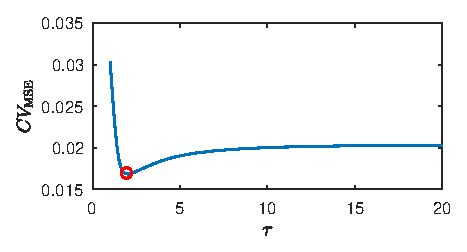
\includegraphics[width=80mm]{bandWidthTesting}
\caption{Cross-validation mean squared error computed for bandwidths ranging from  $1<\tau<20$. The optimal value is indicated by the red circle.}
\label{fig:bandwidth}
\end{figure}

The next step in the model selection process was feature selection by forward search. The original features ($v$, $A$, and $T$), all 2nd order terms ($A^2$, $v^2$, and $T^2$), 2-way interactions ($Tv$, $TA$, $Av$), and the 3-way interaction were considered. As features were sequentially added to the model, $CV_{\hbox{\scriptsize MSE}}$ was used as the selection criteria. For models containing a model specific parameter (e.g. $\tau$, $\lambda$, or $K$), parameter and feature selection occurred concurrently so all combinations of the model parameter and selected features were considered. $CV_{\hbox{\scriptsize MSE}}$ resulting from the WLS feature selection process is plotted in Figure~\ref{fig:CVerror}. Forward search was applied while enforcing the hierarchical principle, which states that if an interaction or high order term is added to a model, then so should the main features involved \cite{friedman2001}. All original features were forced into the model.

\begin{figure}
\centering
 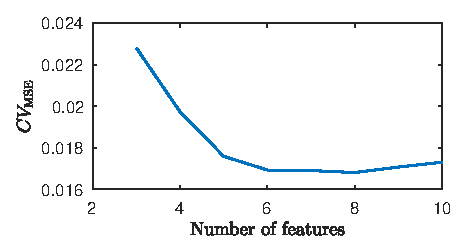
\includegraphics[width=80mm]{featureSelectionWLS}
 \caption{Cross-validation mean squared error as a number of features identified by forward search for WLS.}
\label{fig:CVerror}
 \end{figure}

\section{Regression Models}
\label{regression}
Predicting volume as a continuous random variable is required to instruct users on when to stop adding a particular ingredient. 6 regression models were developed and tested on the training data, including 1) the physical model (Equation~(\ref{eq:2})), 2) ordinary least squares regression (OLS), 3) WLS, 4) Ridge regression, 5) Lasso regression, and 6) K-nearest neighbors. $\alpha$ in the physical model was selected by minimizing the cost function
\begin{equation} \label{eq:7}
J\left( \alpha \right) = \sum_{i=1}^{m} \left( y^{i} - \alpha v^{i}A^{i}T^{i} \right)^{2}\\.
\end{equation}
Differentiating Equation~(\ref{eq:7}) with respect to $\alpha$, setting equal to zero, and solving gives
\begin{equation} \label{eq:9}
\alpha = \frac{\sum_{i=1}^{m} y^{i} v^{i}A^{i}T^{i}}{\sum_{i=1}^{m} (v^{i}A^{i}T^{i})^{2}} \\.
\end{equation}
OLS, Ridge regression, and Lasso regression take the same form as WLS, except the weighting term in Equation~(\ref{eq:4}) is not included, and Lasso ($\lambda = 0.05$) and Ridge ($\lambda = 0.31$) regression are regularized by the 1 and 2 $p$-norm of $\theta$, respectively. Finally K-nearest neighbors predicts $y^{i}$ by averaging the measured volume of the nearest K=6 neighbors (determined from procedure outlined in Section~\ref{mdoel selection}), where distance was defined as the Euclidean distance between the standardized query point and the training observations. All models were developed and implemented using the Statistics and Machine Learning Toolbox$^{\hbox{\small TM}}$ \cite{Matlab}.

The cross-validation root mean squared error ($CV_{\hbox{\scriptsize RMSE}}$) for the training data is shown in Table~\ref{t:regressionDevError}  for all models. $CV_{\hbox{\scriptsize RMSE}}$ is computed from Equation~(\ref{eq:6}) by taking the square root of $MSE^{(i)}$. 95\% confidence intervals for $CV_{\hbox{\scriptsize RMSE}}$ were computed by performing 100 cross-validation trails. Data splitting during the cross-validation step caused $CV_{\hbox{\scriptsize RMSE}}$ to slightly vary. 

The physical model performed worst ($CV_{\hbox{\scriptsize RMSE}}$ = 0.4082 $\pm$ .0002 cup), while WLS preformed best and lead to an error 3 fold lower than the physical model ($CV_{\hbox{\scriptsize RMSE}}$ = 0.1301 $\pm$ .0002 cup). The best-fit WLS model contained 8 features (3 fundamental features, $T^{2}$,$A^{2}$,$AT$,$Av$, and $AvT$). After refitting on all available training data, the WLS model had a RMSE on the test data of 0.1304 cup. Agreement between the training and test MSE suggest the WLS model was not over-fit.

To asses the adequacy of the dataset size for WLS, training data was sub-sampled at different sizes, then split into 70\% training data and 30\% development data. The mean squared error (MSE) between the predicted and actual volume was then computed for both (Figure~\ref{fig:ModelEval}). The training and development errors converge, implying additional data will not improve the WLS fit. For future work, more flexible models could be tested and may potentially reduce the bias error.

\begin{figure}
\centering
 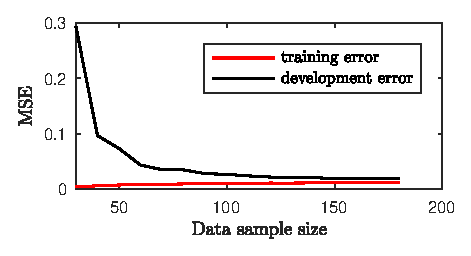
\includegraphics[width=80mm]{dataSampleSizeWLS}
 \caption{Training and development error as a function of dataset size for WLS.}
 \label{fig:ModelEval}
\end{figure}

\begin{table}
\begin{center}
\begin{tabular}{|c|c|}
\hline
 Model & $CV_{\hbox{\scriptsize RMSE}}$ \\ &(cup) \\
\hline
 \multicolumn{1}{|l|}{1) WLS} & 0.1301 $\pm$ 0.0002\\
 \hline
 \multicolumn{1}{|l|}{2) K-Nearest} & 0.1343 $\pm$ 0.0003\\
 \hline
 \multicolumn{1}{|l|}{3) Ridge regression} & 0.1412$\pm$ 0.0002\\
\hline
 \multicolumn{1}{|l|}{4) OLS} & 0.1423$\pm$ 0.0002\\
 \hline
 \multicolumn{1}{|l|}{5) Lasso regression} & 0.1512$\pm$ 0.0002\\
 \hline
 \multicolumn{1}{|l|}{6) Physical model} & 0.4087$ \pm$ 0.0002\\
 \hline
\end{tabular}
\caption{$CV_{\hbox{\scriptsize RMSE}}$ with 95\% confidence intervals computed on the training data for all regression models.}
\label{t:regressionDevError}
\end{center}
\end{table}

\section{Classification Models}
\label{classifcation}
For the recipe-recording, volume classification is required to avoid unmeasurable fractions for future recipe recreation. We developed and compared 5 classification models, each containing 10 categories (1/4 cup increments, from 1/4 to 2 1/2 cups). Tested models included 1) our baseline physical model (Equation~(\ref{eq:6})) rounded to the nearest 1/4 cup, 2) Softmax, 3) K-Nearest Neighbors (KNN), 4) Linear Discriminant Analysis (LDA), and 5) Support Vector Machines (SVM). 
  
Similar to regression model development, the training data were first standardized to have a mean of 0 and variance of 1, and 9-fold cross validation was used to select the best model. For classification, equation 6 was altered by replacing $MSE^{i}$ with the misclassification error $ME^{i}$, where
\begin{equation} \label{eq:10}
ME^{i} = \frac{\sum_{i=1}^{m} 1\left\{y^{i}=\hat{y^{i}}\right\}}{m} \\.
\end{equation}
In the cross-validation procedure 9 folds were applied instead of 10 to ensure each fold contained 2 observations per category. For KNN, the optimal number of neighbors was 3.
 
Development errors for all 5 models are report in Table~\ref{t:regressionDevError}. Softmax performed best. Softmax is a generative learning model that independently predicts categorical probabilities, modeling each posterior distribution as
\begin{equation} \label{eq:11}
p(y=j|x;\theta) = \frac{\exp(\theta^{T}_{i}x)}{\sum_{j=1}^{k} \exp(\theta^{T}_{j}x)} \\.
\end{equation}
The model is derived by finding $\theta$ values that maximize the log-likelihood function
\begin{equation} \label{eq:12}
l(\theta) = \sum_{i=1}^{m}\log\prod_{l=1}^{k} \left (\frac{\exp(\theta^{T}_{i}x)}{\sum_{j=1}^{k} \exp(\theta^{T}_{j}x)}  \right )^{1\left \{y^{i}=1 \right \}} \\.
\end{equation}

\begin{table}
\begin{center}
\begin{tabular}{|c|c|}
\hline
 Model & ME (\%)\\
\hline
 \multicolumn{1}{|l|}{1) Softmax} & 25 $\pm$ 1\\
  \hline
 \multicolumn{1}{|l|}{2) K-Nearest} & 26 $\pm$ 1\\
 \hline
 \multicolumn{1}{|l|}{3) LDA} & 28 $\pm$ 1\\
  \hline
 \multicolumn{1}{|l|}{4) SVM} & 42 $\pm$ 2\\
 \hline
 \multicolumn{1}{|l|}{5) Physical Model} & 78 $\pm$ 3\\
 \hline
\end{tabular}
\caption{$CV_{\hbox{\scriptsize ME}}$ of training data for all models (average of development errors).}
\label{t:regressionDevError}
\end{center}
\end{table}

The feature selection processes for Softmax resulted in 6 features (3 fundamental features, the 3-way interaction term, $T^{2}$, and $v^{2}$).
After fitting on all available training data, the test misclassification error was 25\%. Categorical performance is shown in the confusion matrix presented in Table~\ref{t:confusion}.

\begin{table}
\centering
\begin{tabular}{c|c|c|c|c|c|c|c|c|c|c|}
%\multicolumn{9}{r}{Predicted\, \,} \\[1ex]
  \multicolumn{1}{c}{\,} & \multicolumn{1}{c}{$\frac{1}{4}$}& \multicolumn{1}{c}{$\frac{2}{4}$}& \multicolumn{1}{c}{$\frac{3}{4}$}& \multicolumn{1}{c}{$\frac{4}{4}$}& \multicolumn{1}{c}{$\frac{5}{4}$}& \multicolumn{1}{c}{$\frac{6}{4}$}& \multicolumn{1}{c}{$\frac{7}{4}$}& \multicolumn{1}{c}{$\frac{8}{4}$}& \multicolumn{1}{c}{$\frac{9}{4}$}& \multicolumn{1}{c}{$\frac{10}{4}$} \\[1ex] \cline{2-11}
\multicolumn{1}{c|}{\rule{0pt}{3ex} $\frac{1}{4}$} & \cellcolor{blue!50} 2 & 0& 0& 0& 0& 0& 0& 0& 0& 0 \\[0.5ex] \cline{2-11}
\multicolumn{1}{c|}{\rule{0pt}{3ex} $\frac{2}{4}$} & 0 & \cellcolor{blue!50} 2& 0& 0& 0& 0& 0& 0& 0& 0 \\[0.5ex] \cline{2-11}
\multicolumn{1}{c|}{\rule{0pt}{3ex} $\frac{3}{4}$} & 0 & 0& \cellcolor{blue!50} 2& 0& 0& 0& 0& 0& 0& 0 \\[0.5ex] \cline{2-11}
 \multicolumn{1}{c|}{\rule{0pt}{3ex} $\frac{4}{4}$} & 0 & 0& 0& \cellcolor{blue!50} 2& 0& 0& 0& 0& 0& 0 \\[0.5ex] \cline{2-11}
 \multicolumn{1}{c|}{\rule{0pt}{3ex} $\frac{5}{4}$} & 0 & 0& 0& \cellcolor{red!25} 1& \cellcolor{blue!25}1& 0& 0& 0& 0& 0 \\[0.5ex] \cline{2-11}
\multicolumn{1}{c|}{\rule{0pt}{3ex} $\frac{6}{4}$} & 0 & 0& 0& 0& 0& \cellcolor{blue!50} 2& 0& 0& 0& 0 \\[0.5ex] \cline{2-11}
\multicolumn{1}{c|}{\rule{0pt}{3ex} $\frac{7}{4}$} & 0 & 0& 0& 0& 0& 0& \cellcolor{blue!50} 2& 0& 0& 0 \\[0.5ex] \cline{2-11}
\multicolumn{1}{c|}{\rule{0pt}{3ex} $\frac{8}{4}$} & 0 & 0& 0& 0& 0& 0& 0& \cellcolor{blue!25} 1&  \cellcolor{red!25} 1& 0 \\[0.5ex] \cline{2-11}
\multicolumn{1}{c|}{\rule{0pt}{3ex} $\frac{9}{4}$} & 0 & 0& 0& 0& 0& 0& 0&  \cellcolor{red!50} 2& 0& 0 \\[0.5ex] \cline{2-11}
\multicolumn{1}{c|}{\rule{0pt}{3ex} $\frac{10}{4}$} & 0 & 0& 0& 0& 0& 0& 0& 0&  \cellcolor{red!25} 1& \cellcolor{blue!50} 1 \\[0.5ex] \cline{2-11}
  \end{tabular}
  \caption{Confusion matrix: rows (actual volume) and columns (predicted volume). Results of Softmax test data prediction.}
\centering
\label{t:confusion}
\end{table}

\section{Conclusions and future work}
After guided model development and feature selection, regression and classification models performed better than crude physics-based estimates for volume prediction. Regression test RMSE:  0.13 cups (WLS) vs. 0.41 cups (Physical). Classification test ME: 25\% (Softmax) vs. 75\% (Rounded Physical). Although only 183 observations were available for model development, data sample size testing indicated additional data would not increase prediction accuracy for the simple models tested.

Non-parametric models outperformed parametric models. While all models lead to reasonably low prediction errors, we our not yet ready to advocate for seed funding from the Sandhill VC's. Increased accuracy and environmental adaptability would make the prediction more robust. Ideas for future efforts include 1) testing additional models such as Neural Networks (requires first enslaving undergraduates for additional data collection), Principal Component Analysis combined with various models, and boosted regression trees, 2) improving the current experimental setup by using stereo cameras for a 2D perspective of the flow, 3) improving the feature extraction algorithm to estimate a time varying flow rate and a more rigorous removal of erroneous cross-sectional area values, and 4) expanding the smart device's abilities by generalizing to different environments and measuring dry ingredients and clear liquids.
  
In the end, we had fun, and we learned a lot. Thanks for the class!
  
  
\section{Contributions}
Together:
\begin{itemize}
\item Designed, setup and conducted experiments 
\item Prepared project proposal, milestone, poster, and final write-up
\end{itemize}

Sam's Individual Contributions:
\begin{itemize}
\item Wrote code for edge detection (used for front speed), and length scale extraction.
\item Developed and tested Softmax, weighted linear regression, KNN (Regression and Classification) models. 
\end{itemize}

Kurt's Individual contributions:
\begin{itemize}
\item Wrote code to extract pour duration, front velocity and pixel to length conversion.
\item Conducted data quality check after feature extraction.
\item Developed and tested physical model, OLS, Ridge, Lasso, WLS, and LDA models.
\item Wrote code to test data sample size.  
\end{itemize}

\section{References} 
\bibliographystyle{apalike} 
\bibliography{Bibliography}
\end{document}